\chapter{Study Design and System Implementation}
\label{chapter:studysetting_conduction}
\section{Study Design}
\subsection{Independet Variables: Visual Perspectives}
The last chapter pointed out five possible visual perspecitves in a scenario with one teacher and one student, compare figure~\ref{fig:perspectives}. All visual perspectives are worth an investigation and a comparable study with all five visual perspectives is desirable. Though, to reduce complexity and the number of participants\footnote{Due to COVID-19 pandemic}, this work will focus on three visual perspectives.\\
Figure~\ref{fig:perspectives} shows three main classes of visual perspectives: ego-centric, exo-centric and combinations of them. To answer the research question, it is indispensably to examine at least one of each class. The ego-centric VP is unique and though choosen by default. The exo-centric VP can be realised as purely exo-centric or augmented exo-centric. The combination of ego-centric and exo-centric can be realised as ego \& exo-centric or ego \& augmented exo-centric. But before the exo-centric vp and the combination can be chosen, a closer look on the mechanics that makes Motor Learning in VR possible is necessary.

\subsubsection{Excursion: Mechanics for Motor Learning in Virtual Reality}
For teaching movments in Virtual Reality, in the exo-centric visual perspective the following issue arises. The guidance visualisation can move out of the field of view of the learner by the movement itself. Szenario: the learner and the guidance visualisation stand side-by-side, the learner sees the guidance visualisation on the left of him/her. The guidance visualisation now indicates a movement to turn by 90 degrees to the right. When the learner follow this movement, the guidance visualisation will be located behind the learner after the movement ended. A guidance visualisation standing behind the learner cannot be seen by the learner.\\
This issue is solved in existing work with either the restriction of movements~\cite{freethrowsimulator,elearningma} or multiple representations of the guidance visualisation arround the learner~\cite{thaichichua,mythaichicoaches}. The restriction of movements has an strong influence in the task design and is therefore not desirable for the study proposed in this thesis. Consequentially, for exo-centric visual perspectives multiple representations for the guidance visualisations on strategic positions arround the learner are necessary.\\
In the ego-centric visual perspective, another issue araises during the teaching of locomotion movements. To understand this issue, two aspects have to be clear before. (1) The nature of an ego-centric guidance visualisation is to be located inside the learner at any time. (2) A guidance visualisation indicates movements by moving itself. If the guidance visualisatoin is about to indicate a movement away from the learner, the guidance visualisation is moving out of the students body. But a guidance visualisation that is outside of the learners body is no longer ego-centric.\\
A possible soltuion can give the centricity continuum by Wang and Milgram~\ref{fig:ego-exo-continuum}. Following the nature of the centricity continuum, the tethering distance can be increased by a small ammount and the visual perspective can still be classified as ego-centric. But now araises the question, of how far the tethering distance can be increased, with which the perspective still feels ego-centric, but the indication of the movement is considerable. For simplicity reasons, this distance is further called ego-centric tethering distance (ETD). To determine a reasonable ETD, a small formative study was conducted\footnote{A larger study was not possible because of the COVID-19 pandemic}. During this study, a non biased\footnote{The person had no prior knowledge about the system or motor learning.} person was asked to follow movements in the ego-centric visual perspective. The first movement was conducted with an ETD of 5cm. For the folowing movements the ETD was increased by 5cm each. The subjective assesment of the participant and my observations yielded best for an ETD between 15cm and 30cm. These two values are further called:
\begin{itemize}
	\item[] $ETD_{min}=15cm$
	\item[] $ETD_{max}=30cm$
\end{itemize}
Based on $ETD_{min}$ and  $ETD_{max}$ the speed mechanic is developed. The speed mechanic controls the speed of the playback of the guidance visualisation. At $ETD_{min}$ and below, the animation plays at normal speed. At $ETD_{max}$ the guidance visualisation stops. Between $ETD_{min}$ and $ETD_{max}$ the animation speed of the guidance visualisation is linearly interpolated, compare figure~\ref{fig:speed_mechanic}.
\begin{figure}[htb]
	\centering
	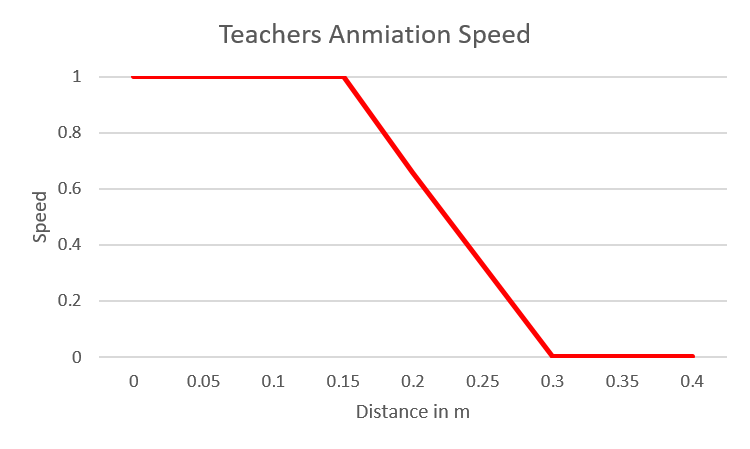
\includegraphics[width=\textwidth]{figures/speed_mechanic_chart.png}
	\caption[speed mechanic chart]{speed mechanic chart}
	\label{fig:speed_mechanic}
\end{figure}
The speed mechanic was evaluated by one person\footnote{Different person than the first one. This person had no prior knowledge about the system nor Motor Learning. A Larger evaluation was not possible because of COVID-19 pandemic.}. The participant followed the guidance visualisation in the ego-centric visual perspective. Observations showed that the participant could follow the movement at ease. The opinion of the participant about the speed mechanic was very positive.\\
With this short excursion, a reasonable decision for the exo-centric VP and the combination can be chosen.\\
\hspace{1cm}

In the ego-centric visual perspective, the learner sees the guidance visualisation inside the own body. Here, the learner can see the relation of the own body to the GV directly. In the pure exo-centric visual perspective this relation cannot be seen. Thereby, the position of the learner in relation to the guidance visualisation must be guessed. That, in turn, makes the application of the speed machanic - which is necessary for ego-centric guidance - not possible. A mechanic that is used in all conditions but one could lead to biased data, compare table~\ref{tab:mechanics}.
\begin{table}[htb]
	\centering
	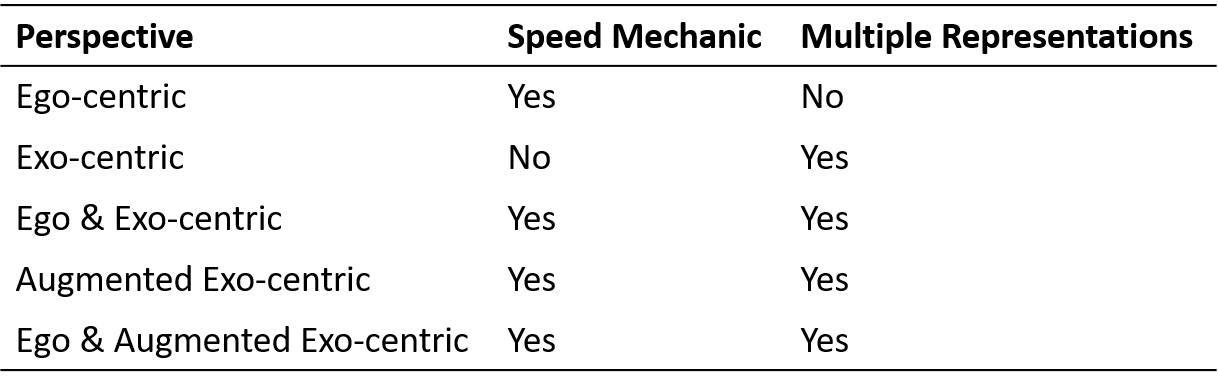
\includegraphics[width=\textwidth]{figures/mechanics_comparison.png}
	\caption[Mechanics for Motor Learing in Virtual Reality]{Mechanics speed and multiple representations and in which VP they are applied.}
	\label{tab:mechanics}
\end{table}
The mechanic of multiple representations does not influence the validity of the study, because the mechanic would solve an issue that does not exist in the ego-centric perspectives.\\
In the augmented exo-centric perspective, a virtual copy of the learner is located inside the exo-centric guidance visualisation. The copy lets the learner see the relation of the own body to the guidance visualisation. Furthermore, augmenting the exo-centric guidance visualisation with the learner is widely used and evaluated in related work~\cite{YouMove,thaichichua}. Consequently, the augmented exo-centric VP will serve as the exo-centric VP.\\
With the ego-centric and exo-centric VP set, the combination can be chosen. In the ego-centric VP the learner has a direct comparison of the own posture to the posture of the GV in the ego-centric VP. In the augmented exo-centric VP the learner has a direct comparison of the own posture and the posture of the GV in the exo-centric VP. To have the direct comparison from the ego-centric VP AND the exo-centric VP, the ego \& augmented exo-centric VP is chosen as the combination. The ego \& augmented exo-centric VP is the true combniation of ego-centric and augmented exo-centric.\\
For simplification, the augmented exo-centric VP will be further called exo-centric VP, and the ego \& augmented exo-centric will be further called ego \& exo-centric VP.\\
The ego-centric VP, exo-centric VP and the ego \& exo-centric VP are the independent variables of the study and form the three study conditions EGO, EXO, EGO \& EXO.

\subsection{Measures: dependent variables}
This works aim is to answer the main researchquestion RQ1: How does the visual perspective on a virtual guidance visualisation influence Motor Learning in Virtual Reality. To answer this research question, the proposed study has to generate data that ansers the sub-research questions RQ1.1-4. This section will provide the underlying paradigma to every sub-research question and explain which measures are necessary.

\begin{itemize}
	\item[] \textbf{RQ1.1} How does the visual perspective on a virtual guidance visualisation influence movements' accuracy?
	\begin{itemize}
		\item[] \textbf{RQ1.1.1} How does the visual perspective on a virtual guidance visualisation influence movements' accuracy of the own body?
		\item[] \textbf{RQ1.1.2} How does the visual perspective on a virtual guidance visualisation influence the accuracy of handling physical load?
		\item[] \textbf{RQ1.1.3}How does the visual perspective on a virtual guidance visualisation influence sub-tasks' accuracy?
	\end{itemize}	
	\item[] \textbf{RQ1.2} Does the visual perspective on a virtual guidance visualisation influence the transfer of ergonomic principles?
	\item[] \textbf{RQ1.3} How does the visual perspective on a virtual guidance visualisation influence the learner's visual focus?
	\item[] \textbf{RQ1.4} What is the subjective personal preference of the learner for the visual perspectives?
\end{itemize}

\subsection{Task Design}
The task design for the proposed study founds on this basis and additionally should have a reference to real-world tasks. For the task, a simple box serves as physical load, compare chapter \todo{3}.\\
The real world provides a variety tasks that include the handling of physical load. For example in a pacel transhipment point, wearhouse workers, grinders or people that work at test stands. They pic up physical load, carry, turn and pull it. To imitate such a task, additional artifacts were created to be used in the proposed study. A table for push and pull, that could be interpreted as a machine or sorting platform and a plate on the floor that could depict for example a scale. Between the table and the scale the box can be carried. The box can be lowered and lifted from and to the scale.\\
As described in chapter \todo{4}, the legs during push and pull are in the same position if executed ergonomically. To gain variation, which is necessary to get insight how the learner can see the feet of the guidance visualisation, two non-elemental tasks were introduced: turn and fold. During this task the foot placement is different to push and pull. With the sub-tasks lift, lower, push, pull, carry, turn and fold the first task was designed. It consisted out of 28 sub-tasks were every sub-task occured 4 times. During the design of the task became clear that an additional element had to be introduced: walking. This enables more variation in the task. For example, the task executer stands at the left side of the table and pushes the box away. Now the executor can walk to the left side and pull the box.


Lift and lower can be realised by lifting the box from the floor and lower the box to the floor. For push and pull, another artifact is necessary: a table makes the execution of push and pull easier than on the ground.


manual material handling~\cite{mmh}, single: lift lower push pull carry hold, hold out because of confusion with speed mechanic, introduced carry because of variaation and flexibility in task. unit/combined mmh tasks classification.\\
baua classification?
%https://www.baua.de/EN/Topics/Work-design/Physical-workload/Types-of-workload/Types-of-workload_node.html https://www.baua.de/DE/Themen/Arbeitsgestaltung-im-Betrieb/Gefaehrdungsbeurteilung/Expertenwissen/Physische-Belastung/Heben-Halten-Tragen/Heben-Halten-Tragen_node.html



\subsection{How to Evaluate}
\subsection{Procedure}
\subsection{Research Contribution Statement}
\label{delimination_contribution}
The conduction of the proposed study will produce data that serves as a reasonable basis for designers of VR Motor Learning systems choosing a suitable perspectives. This is achieved by an Empirical Research Contribution. The empirical data is gathered by a comparative study between the ego-centric visual perspective, the exo-centric visual perspective and the combination. As novelty, the task includes handling of physical load which consists of the elemental tasks of manual material handling. This allows an evaluation of the elemental tasks per visual perspective and can give insights which perspective is suited for specific tasks.\\
Additionaly, an artifact contribution is provided by the ego-centric guidance of locomotion movements.
\section{\exgo - Design and Implementation}
(15 pages)
\section{\exgo}
\label{section:system}
\subsection{Study Setting}
Studysetup\\
frameworks\\
implementation\\
perspectives\\
mechanics\\
logging\\
limitations\\
iterative implementation\\
formative tests\\
\section{Study}
\label{section:study}

\begin{figure}[htb]
	\centering
	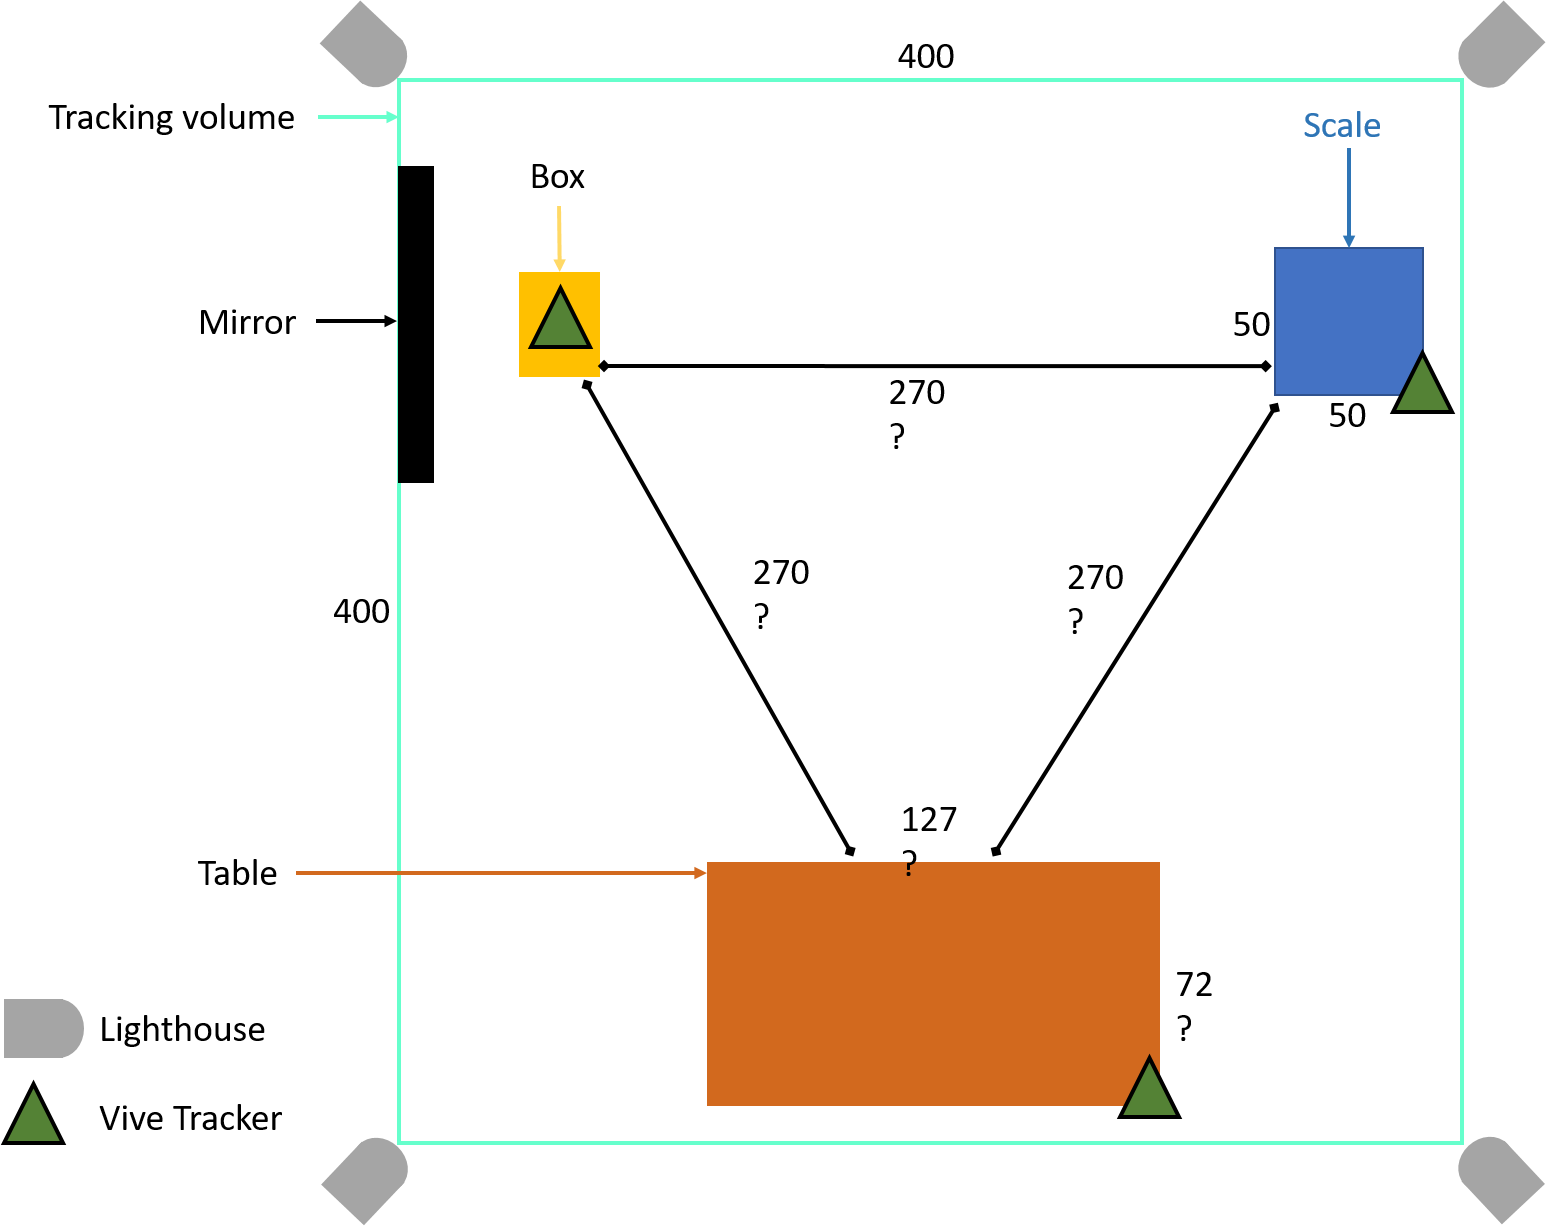
\includegraphics[width=\textwidth]{figures/study_setting.png}
	\caption[study setting]{study setting}
	\label{fig:study_setting}
\end{figure}

\begin{figure}[htb]
	\centering
	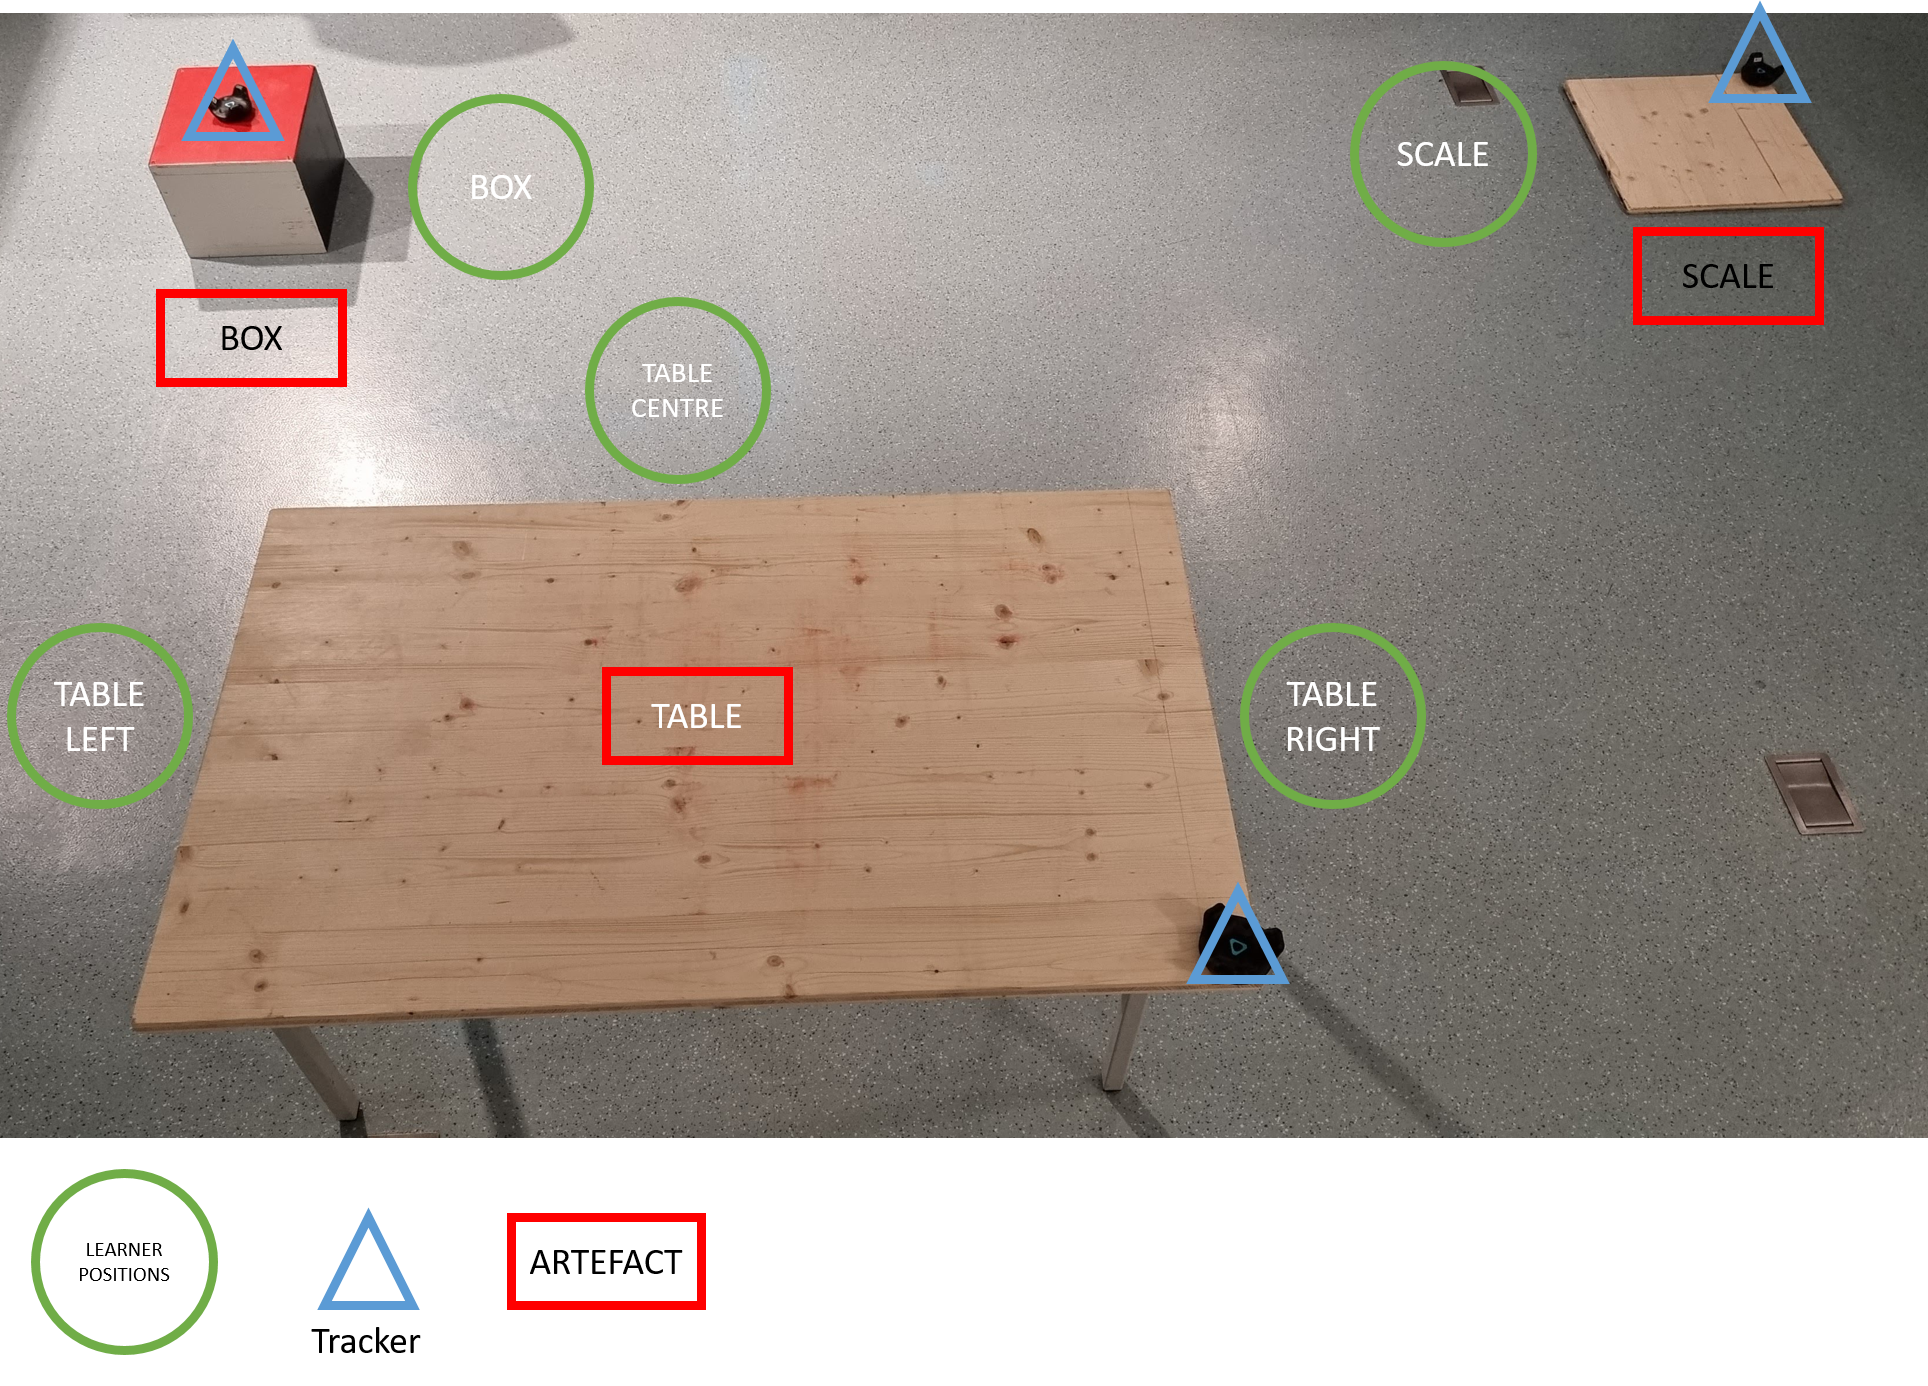
\includegraphics[width=\textwidth]{figures/learner_positions.png}
	\caption[Description of tasks]{tasks}
	\label{fig:learner_positions}
\end{figure}

\begin{figure}[htb]
	\centering
	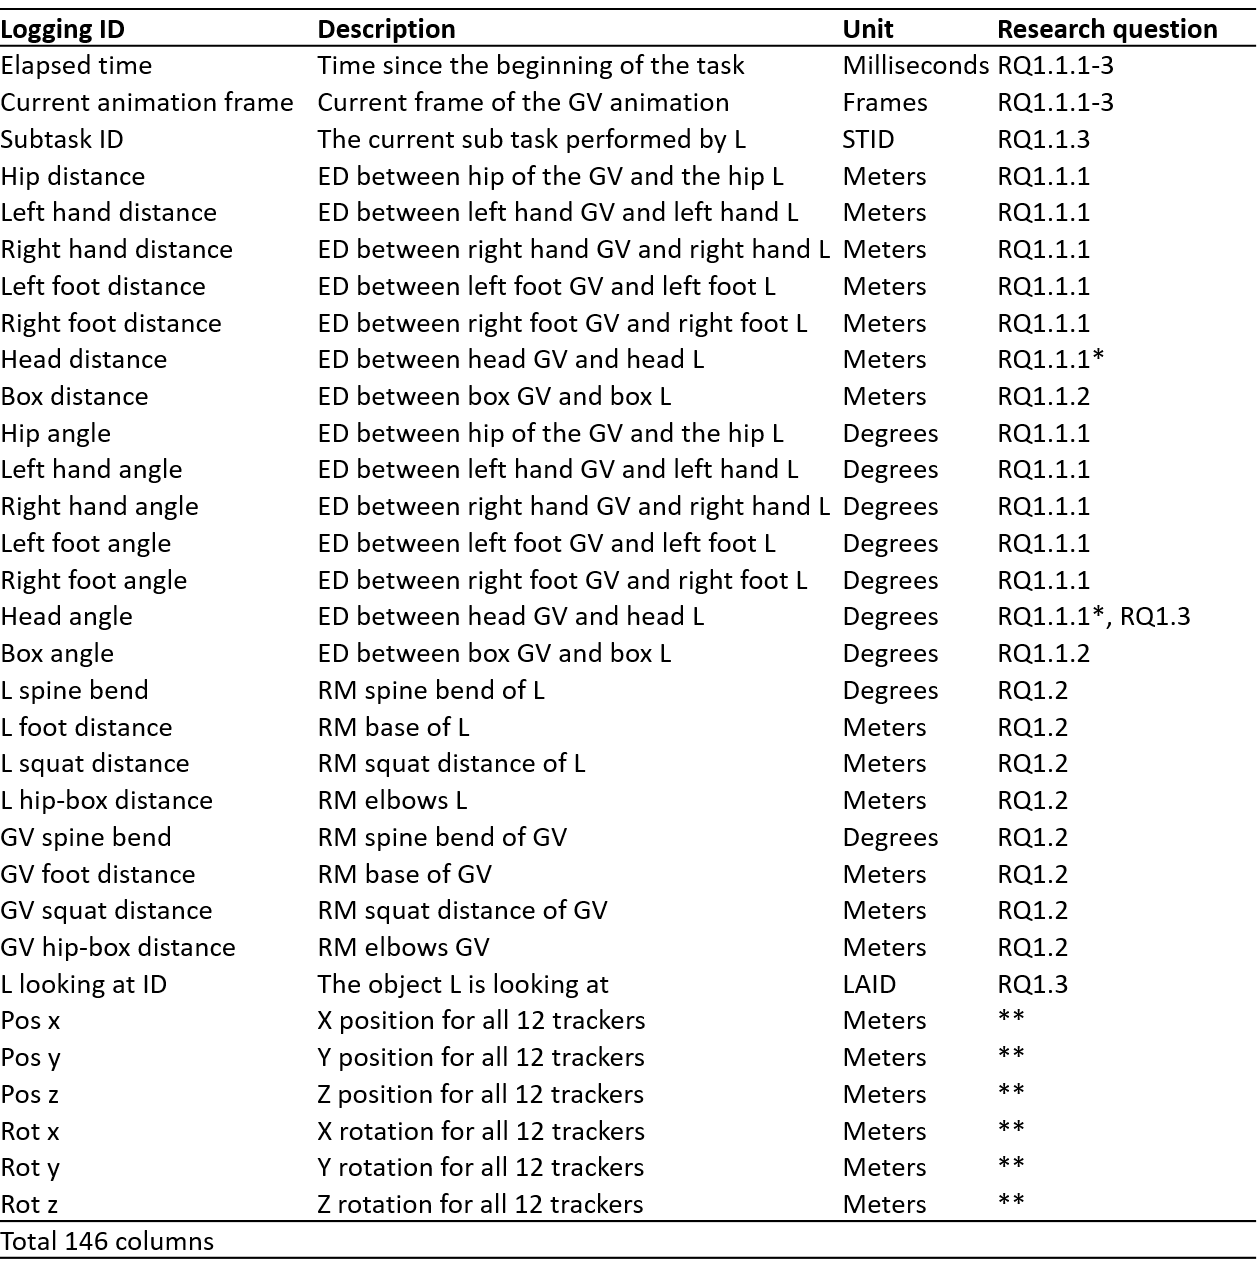
\includegraphics[width=\textwidth]{figures/logging_detail.png}
	\caption[logging detail]{Detailed overview of logs produced by \exgo\ per frame. L: learner, GV guidance visualistion, ED: euclidean distance. *head position and rotation is biased in exo-centric conditions because of multiple GV the L can focus on. **All trackers are logged for backup reasons: after the study is conducted a measurement can become interesting that was not of imporance before. With these values any measurement can be calculated post-study.}
	\label{fig:logging_detail}
\end{figure}

\begin{table}[htb]
	\centering
	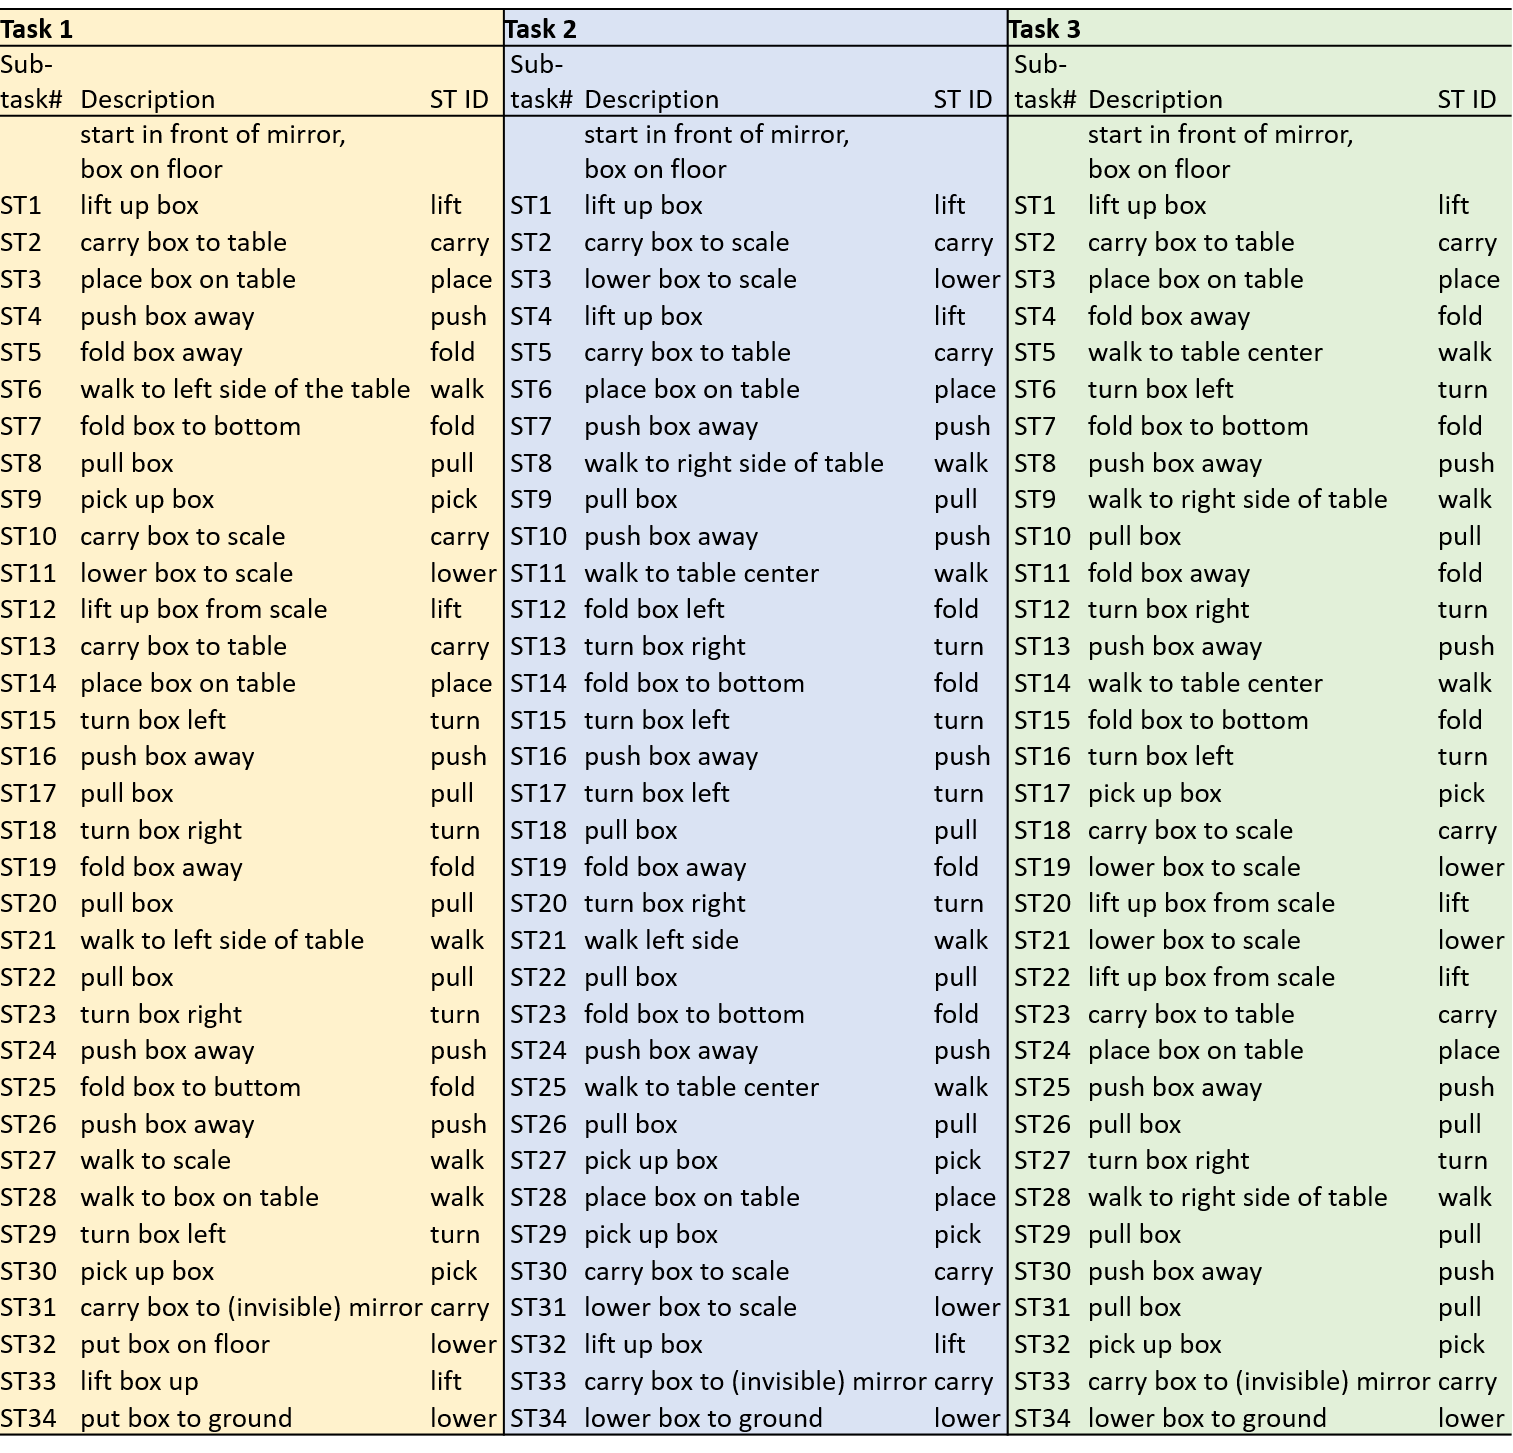
\includegraphics[width=\textwidth]{figures/tasks.png}
	\caption[Description of tasks]{tasks}
	\label{tab:tasks}
\end{table}

\begin{table}[htb]
	\centering
	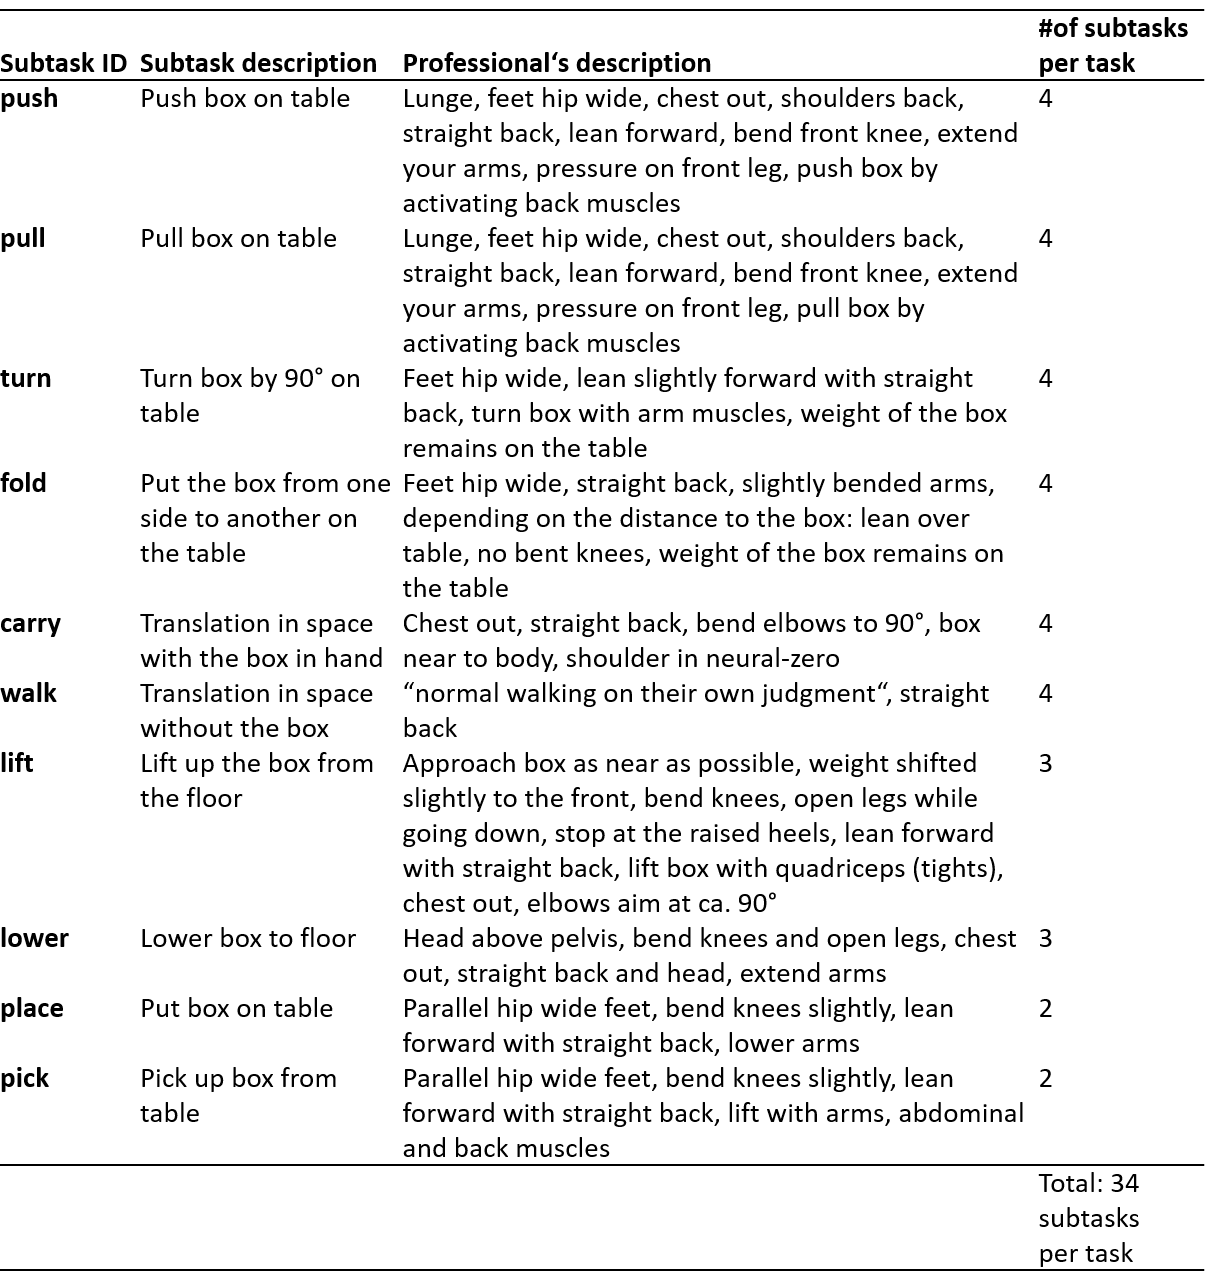
\includegraphics[width=\textwidth]{figures/sub_tasks_definition.png}
	\caption[Description of sub-tasks]{subtasks}
	\label{tab:sub-tasks}
\end{table}

\begin{figure}[htb]
	\centering
	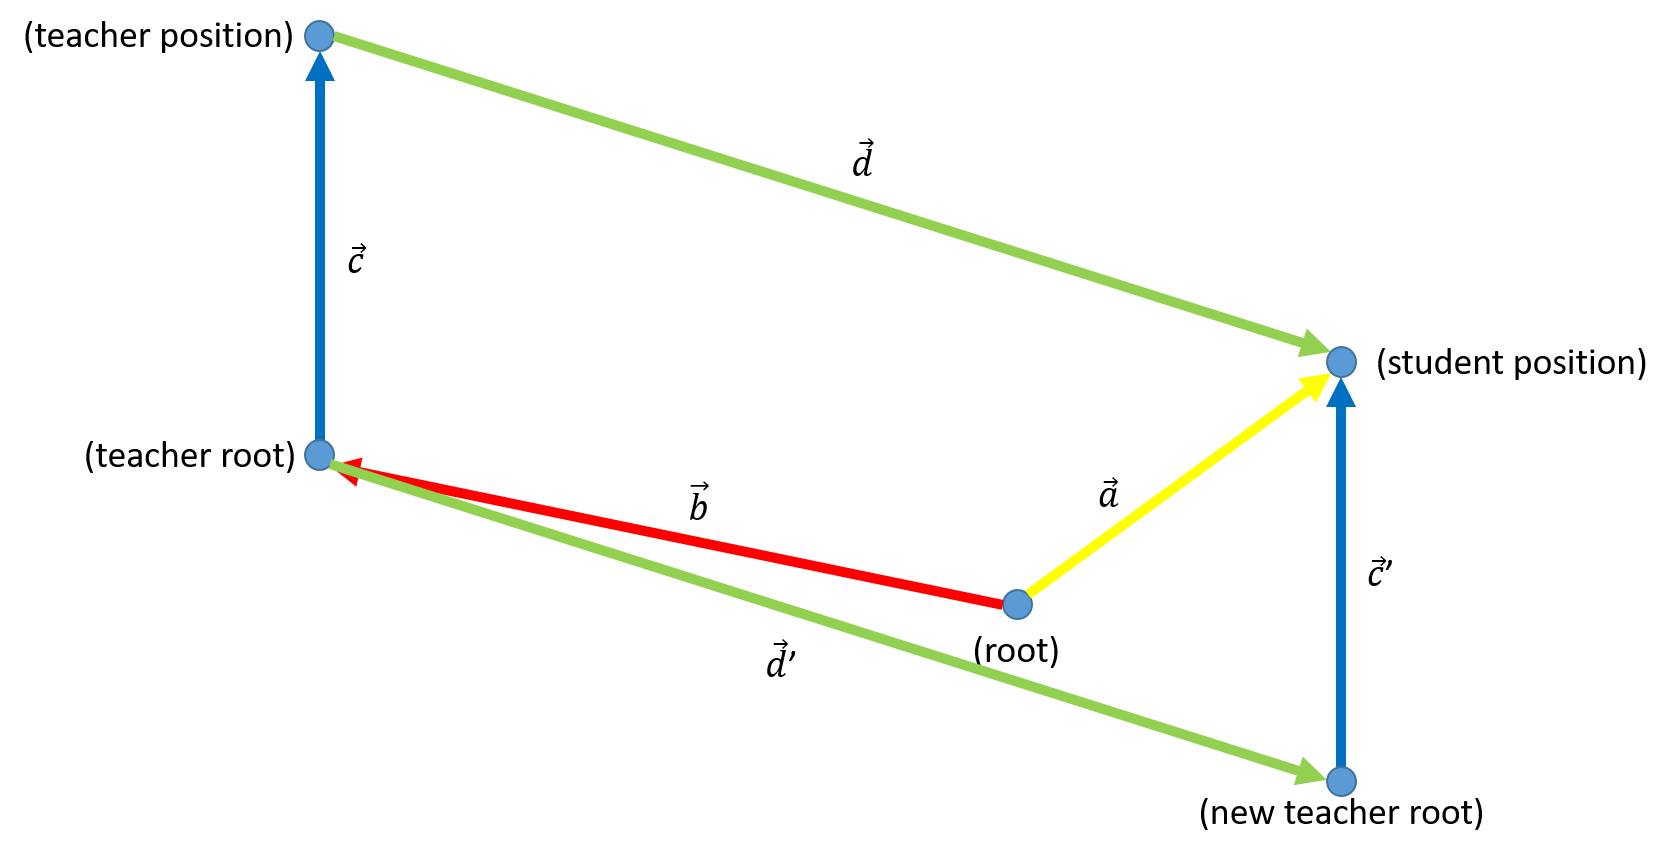
\includegraphics[width=\textwidth]{figures/shift_calc.png}
	\caption[shift calc]{shift calc}
	\label{fig:shift_calc}
\end{figure}



\begin{figure}[htb]
	\centering
	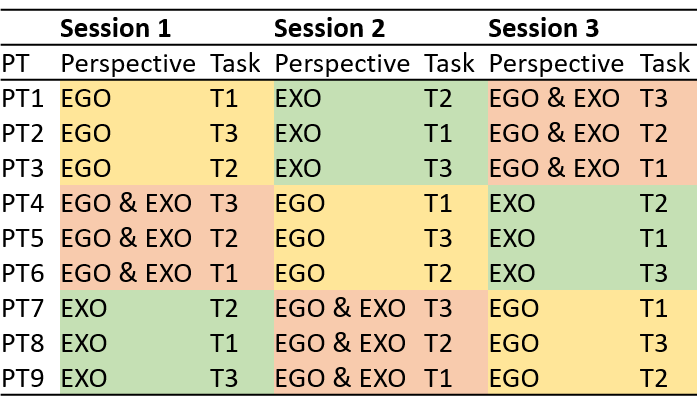
\includegraphics[width=0.5\textwidth]{figures/study_session_plan.png}
	\caption[session plan]{session plan}
	\label{fig:study_session_plan}
\end{figure}

tasks\\
procedure\\
geplante evaluierung\\
limitations\\
bezug zwischen messungen und forschungsfragen\\
triangulation nutzen wo sinnvoll\\
